\documentclass{article}                                                         
\usepackage[utf8]{inputenc}                                                
\usepackage[margin=1in]{geometry}                                           
\usepackage{graphicx}                                                        
\usepackage{subcaption}                                                      
\usepackage{mathtools}                                                       
\usepackage{xcolor}                                                          
\usepackage{parcolumns}                                                     
\usepackage{multirow}                                                       
\usepackage{hyperref}
 \hypersetup{
    colorlinks=true,
    linkcolor=blue,
    filecolor=magenta,      
    urlcolor=blue,
    pdfpagemode=FullScreen,
    }                                                                              

\begin{document}

\noindent
   \begin{titlepage}
    \vspace*{\fill}
    \begin{center}
      {\huge \textbf{ASCII LCD Display} }\\[0.5cm]
       {\LARGE \textbf{User Manual}}\\[0.4cm]
     {\Large Luis D. Garcia}\\[0.4cm]
    \end{center}
     \vspace*{\fill}
   \end{titlepage}
\newpage

\tableofcontents
\thispagestyle{empty}
\cleardoublepage

\setcounter{page}{1}

\section{Product Description}
\noindent
Print any 1-5 letter word on both rows of an LCD display using 8-bit binary numbers. Your 8-bit 
binary number gets converted to its ASCII value, so the LCD can display it is as a letter.
Each letter is inputed individually by using the Basys 3 switches to represent an 
8-bit binary number then sending that number by pressing a button on the Basys 3 to 
the Arduino. The Arduino then converts your 8-bit binary to ASCII and displays the ASCII 
value on the LCD display. Hence, leave messages for a loved one, a visitor, or even an a new acquaintance. 
For instance, a message such as "Howdy there" will be displayed as "Howdy" on the first row of the LCD display and "there"
on the second row of the LCD display due to the 5 letter cap for each row. 

\begin{figure} [ht!]
\centering
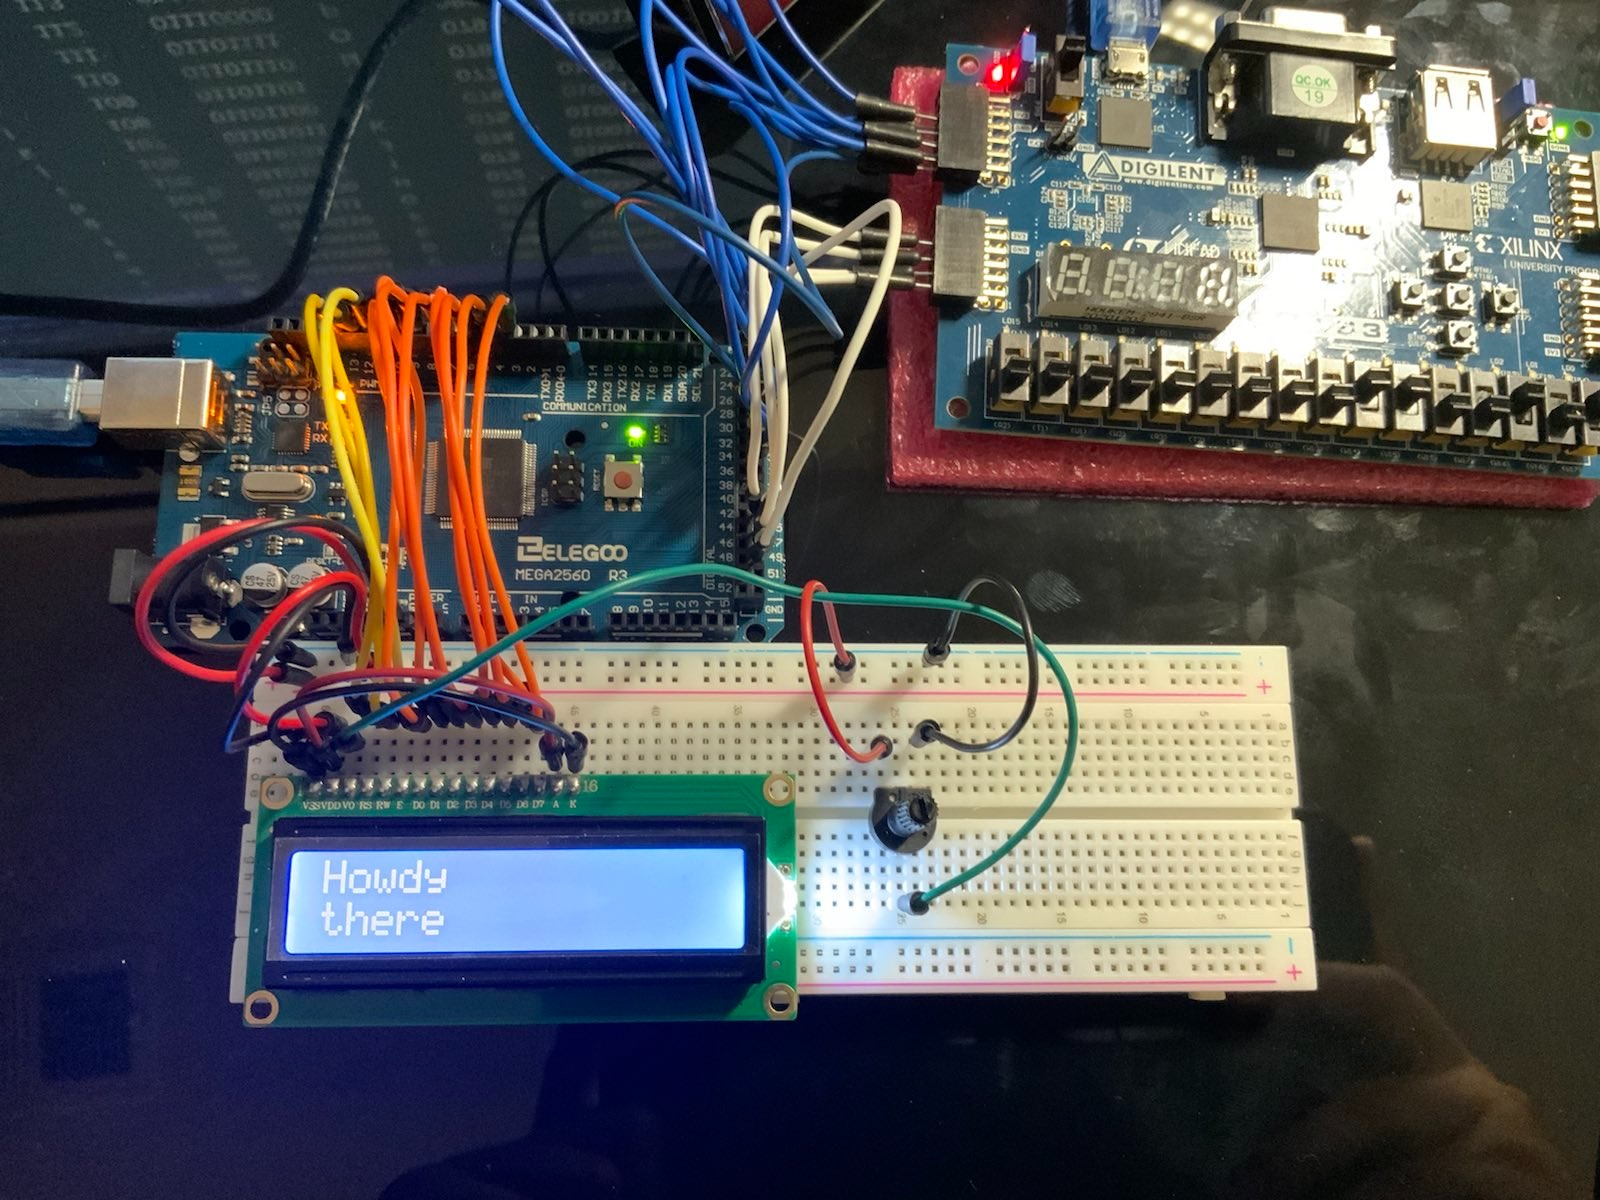
\includegraphics[width=0.6\linewidth]{Howdy.jpeg}
  \caption{An example of How the LCD displays Data}
  \label{fig:fig1}
\end{figure}


When you get tired of seeing the same message just clear the screen by pressing another button then just enter a new message
like you did before.


\section{Set-Up}
\begin{figure} [ht!]
\centering
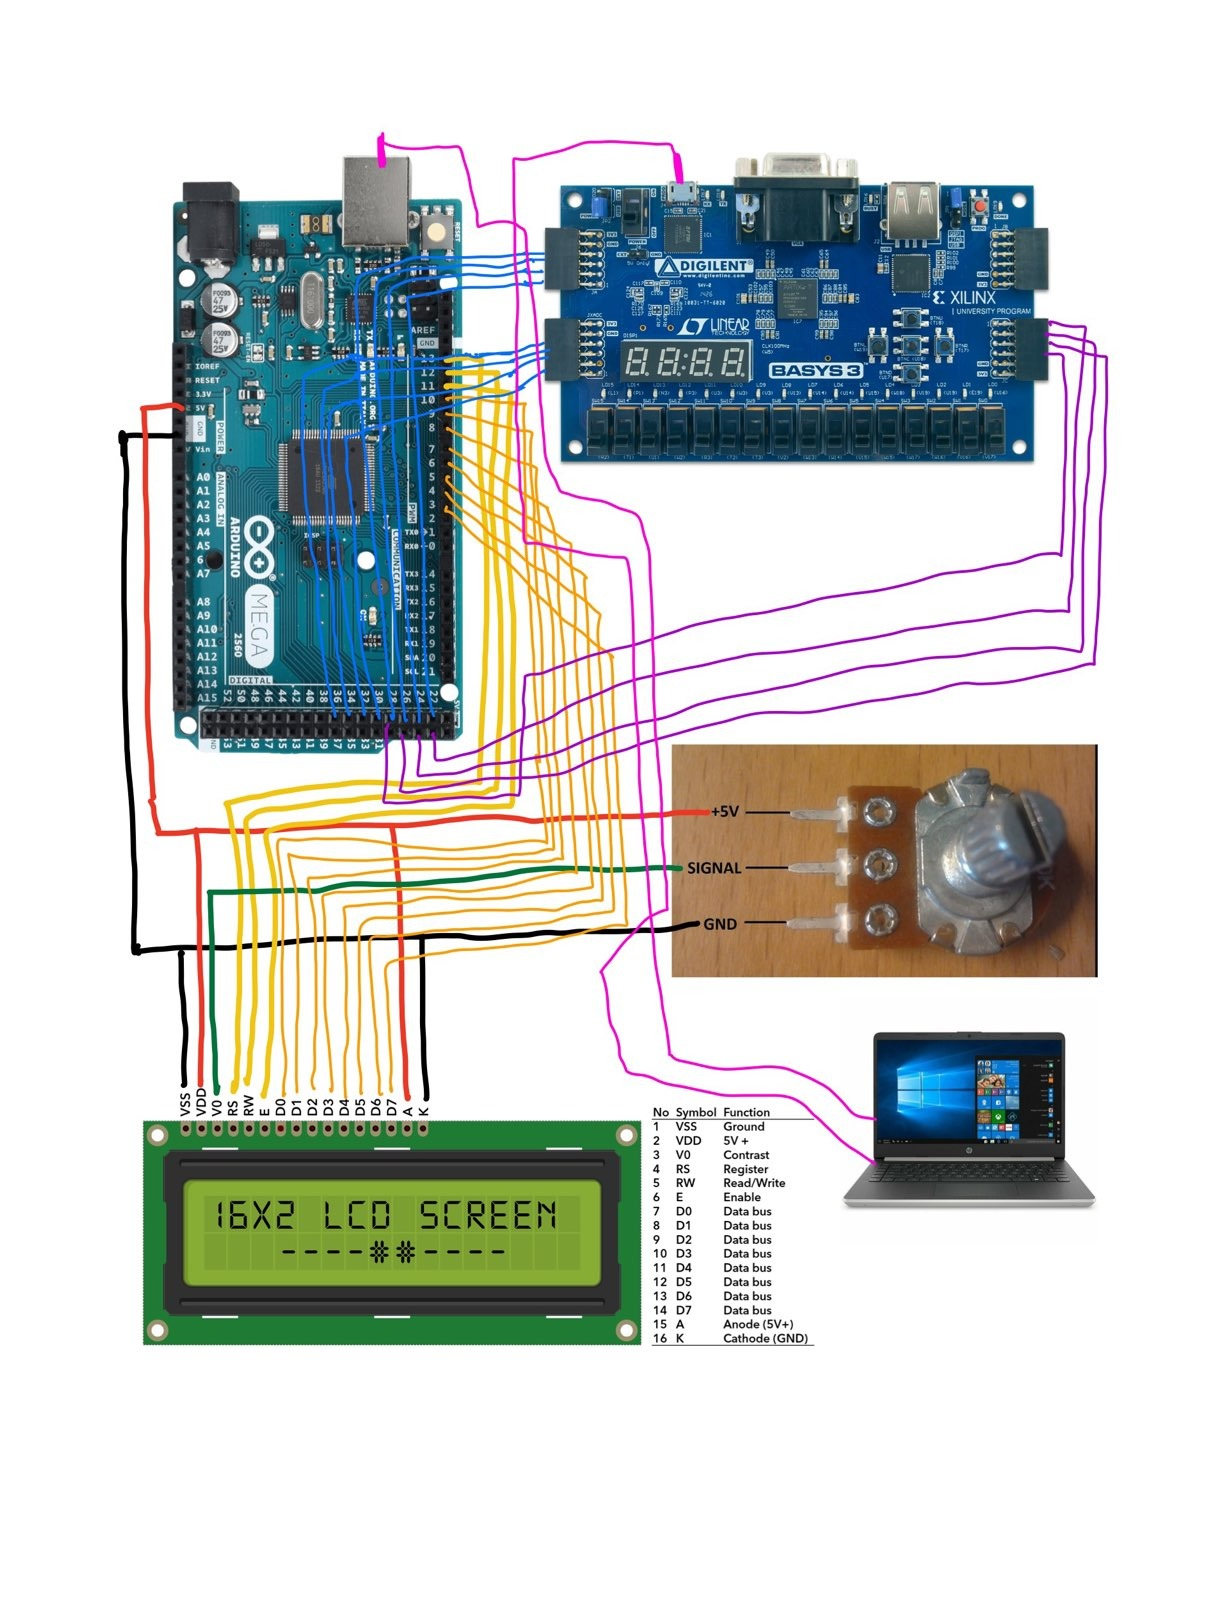
\includegraphics[width=0.9\linewidth]{WireModel.jpg}
  \caption{Wiring Model for Set-Up}
  \label{fig:fig2}
\end{figure}


The components necessary for the set-up are a Basys 3 board, Arduino Mega, wires, potentiometer, 5V LCD 16x2 LCD display, Arduino
USB cable, a breadboard, and micro-USB cable. To begin one should insert the pins of the potentiometer and LCD screen into the 
breadboard and connect them as seen with the red 5V wire,
black ground wire, and green signal wire in Figure 2. Additionally,
connect LCD pins VSS and K to ground and LCD pins VDD and A to 5V. Then 
connect LCD pins RS, RW, and E to pins 13, 12, and 11 in that 
order. Next make the connections for the D inputs (D0-D7) by
putting to them to the corresponding Arduino Mega pins of 10, 9, 8, 7, 6, 5,
4, and 3. Now that you have all the connnections set adjust the potentiometer until your LCD screen appears blue as seen in 
Figure 3. The potentiometer permits you to adjust the screen brightness so that you can see the letters you 
want to output on the screen.

Moreover, on the Basys 3 board the 8 blue wires on Figure 2 must 
connect to 8 digital pins on the Arduino Mega, as these 
wires transmit the data of the 8 rightmost switches 
of the Basys 3. The 4 purple wires in Figure 2 transmit data
from the buttons of the Basys 3 board (top button, left
button, right button, and center button) regarding if they
were pressed or not since these provide the 
LCD instructions to begin reading data and insert data. Finally, insert the Arduino USB cord to a laptop 
that has the code for the design and insert the micro-USB 
to the Basys 3 board and the computer to upload the bitstream
onto the board using Vivado.

\begin{figure} [ht!]
\centering
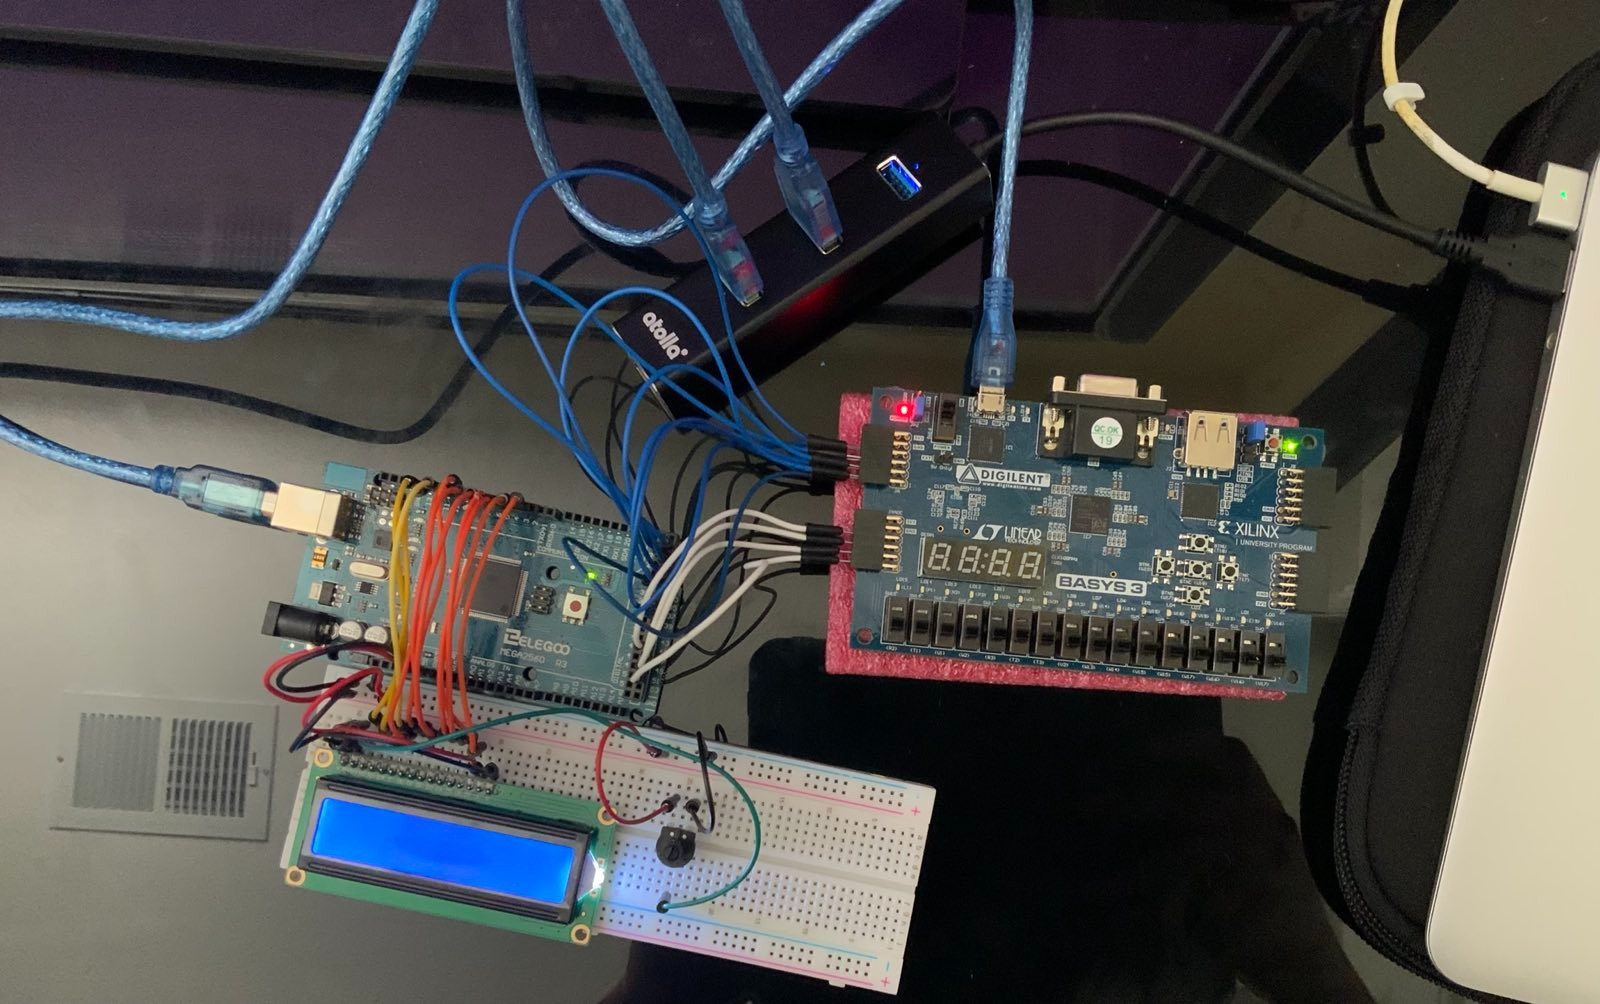
\includegraphics[width=0.7\linewidth]{SetUp.jpg}
  \caption{Successful Set-Up}
  \label{fig:fig3}
\end{figure}

\newpage

\section{How to Use}
\subsection{Enter a Letter}
The first instruction one wants to take after completing the set-up is to input 
a letter such as "a" for the LCD to display. To do this one must 
find the what the binary representation for the ASCII code of "a" is using the 
\href{https://abcfundkids.blogspot.com/2021/11/8-bit-binary-code-alphabet-get-ascii.html}{ASCII-Binary Character Table}.
Then using the switches on Basys 3 board shown in Figure 4 enter the 8-bit 
binary value for the letter you want to input, where the rightmost
switch is the least significant bit and the rightmost bit is the most siginficant
bit. 
Once you have set your switches just push the next letter button as seen in Figure 5 and your letter 
will appear on the LCD screen. 
\begin{figure} [ht!]
\centering
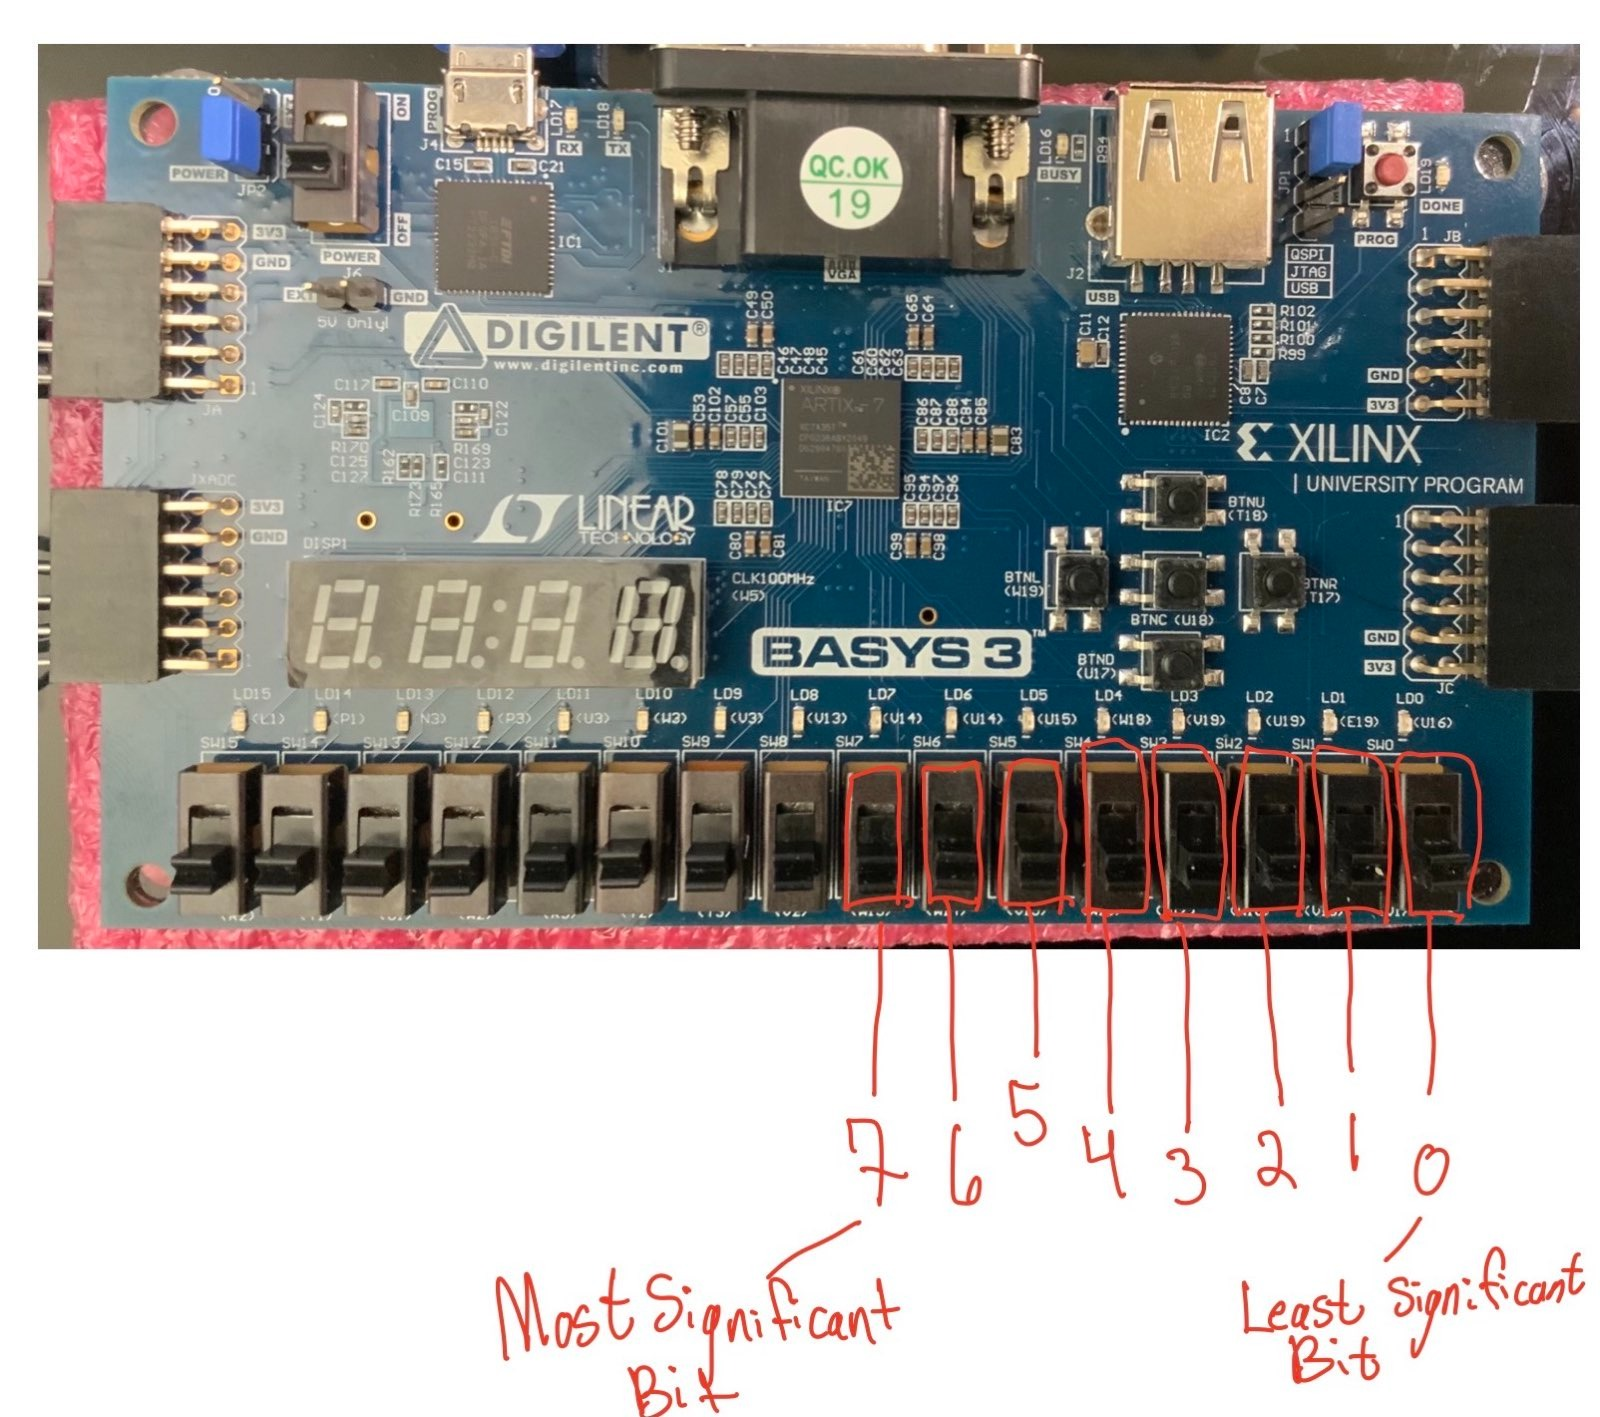
\includegraphics[width=0.7\linewidth]{Switches.jpg}
  \caption{Switches to Use on the Basys 3}
  \label{fig:fig4}
\end{figure}
\newpage

\begin{figure} [ht!]
\centering
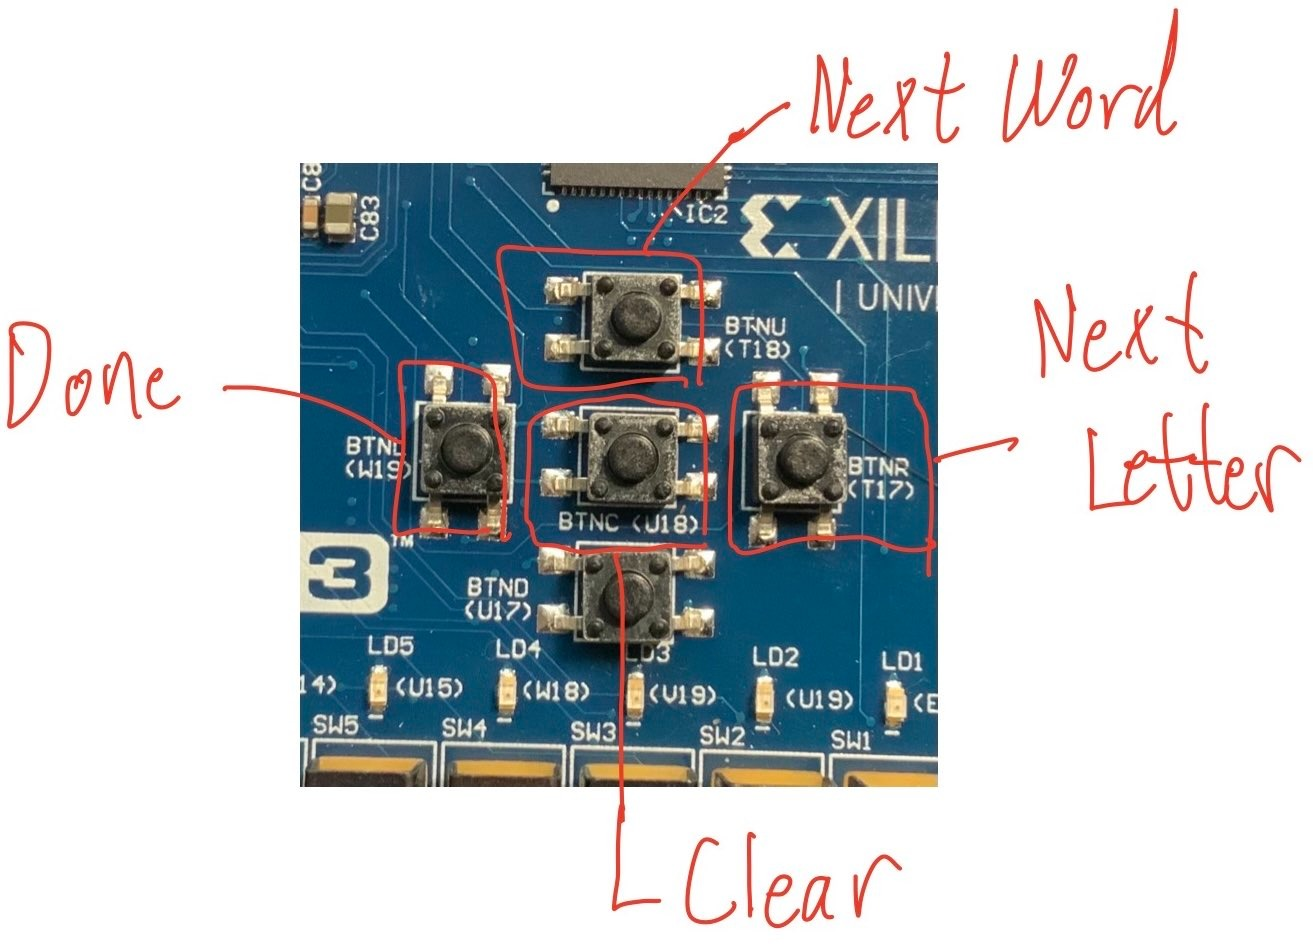
\includegraphics[width=0.7\linewidth]{Buttons.jpg}
  \caption{Buttons to Use on the Basys 3}
  \label{fig:fig5}
\end{figure}
\newpage

As an example if you wish enter the letter "H" then using the switches enter it's 8-bit binary equivalent value,
which is "01001000," as seen in Figure 6. Then after setting your switches press the "Next Letter" button to
have the "H" appear on your screen as seen in Figure 7. If you wish to add any more letters just reset your 
switches to match the 8-bit binary value of the new letter you want to enter and press the "Next Letter" 
button again.

\begin{figure} [ht!]
\centering
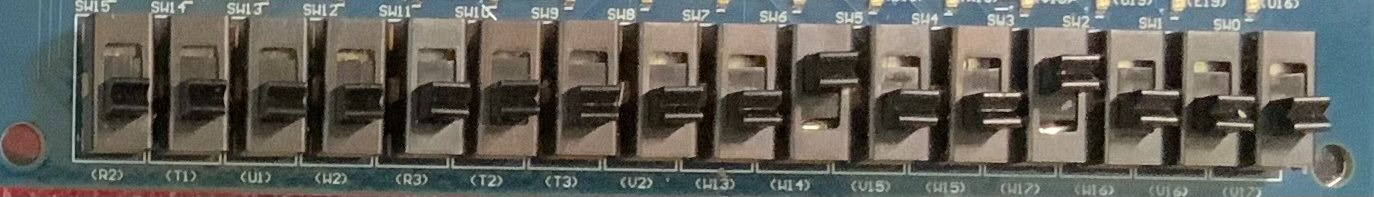
\includegraphics[width=0.7\linewidth]{HBinary.jpg}
  \caption{Switches to Represent H in 8-Bit Binary}
  \label{fig:fig6}
\end{figure}

\begin{figure} [ht!]
\centering
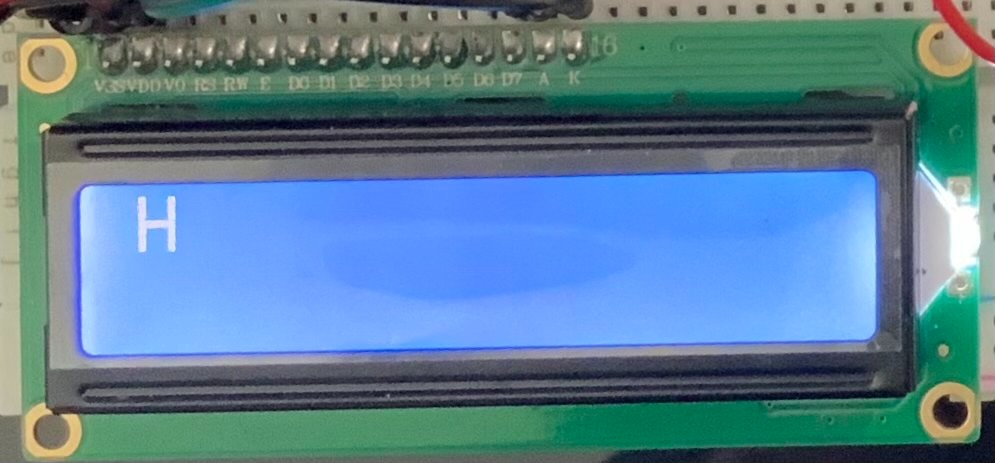
\includegraphics[width=0.7\linewidth]{H.jpg}
  \caption{H being Display on the LCD Screen}
  \label{fig:fig7}
\end{figure}

\subsection{Clear the Display}

When you want to clear your display for whichever reason press the Clear screen button as seen in Figure 5, and you 
will then get a blank blue screen, which indicates the LCD screen is ready to accept any new letters 
you wish to display on the LCD. The result of pressing the Clear screen button is best captured in Figure 8, which 
demonstrates what will occur when the Clear button is pressed.

\begin{figure} [ht!]
\centering
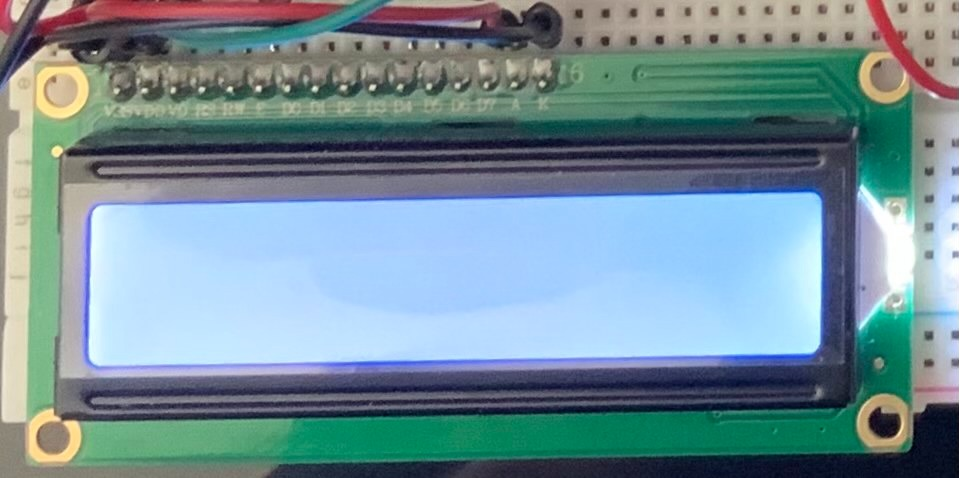
\includegraphics[width=0.7\linewidth]{Clear.jpg}
  \caption{Result of Pressing Clear Screen Button}
  \label{fig:fig8}
\end{figure}

\subsection{Enter a Word Less than 5 Letters}
If you want to create a word less than 5 letters on either the first, second, or both rows of the press the "Next 
Word" button, which adds extra spaces to meet the 5 letter limit. For instance, in Figure 9 the word on the first 
row is "Hi," and the word on the second row is "Dude." In order to get "Hi" to display on the screen enter each
letter that after entering "i" press the "Next Word" button, which will let you enter the letters for the word
"Dude." Once you enter the "e" in "Dude" press either the "Done" or "Next Word" button since both will just add 
an extra space to meet the 5 letter count. 


\begin{figure} [ht!]
\centering
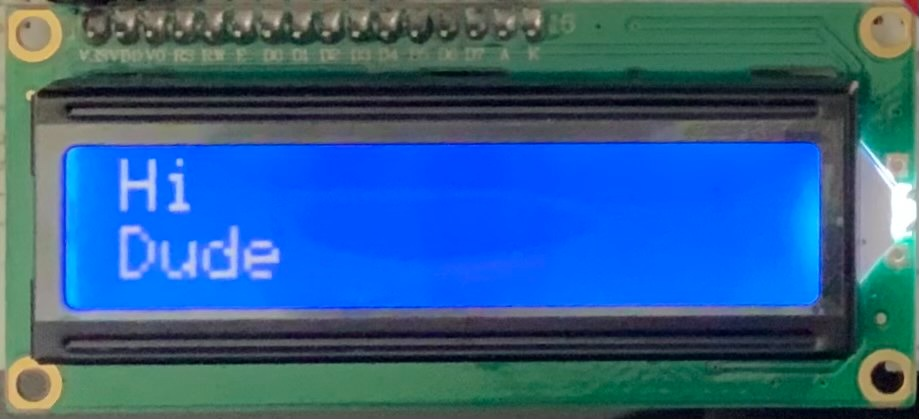
\includegraphics[width=0.7\linewidth]{Less5.jpg}
  \caption{LCD Display of Words Less than 5 Letters}
  \label{fig:fig9}
\end{figure}


\subsection{Enter only One Word}
If you want to enter only one word on the first row of the LCD screen then input the letters you want to create the 
word as you normally would then press the "Done" button seen in Figure 5. For instance, in Figure 10 the word
"Home" is displayed and no other letters can be inputted since the "Done" button was entered, so one must
press the "Clear" button if they want to enter a new letter. However, if you want to create a word only in the 
second row then press the "Next Word" button first and then enter the letters you want to create your second
word. The letters will appear on the second row then just press the "Done" button when you finish adding 
all your letters.

\begin{figure} [ht!]
\centering
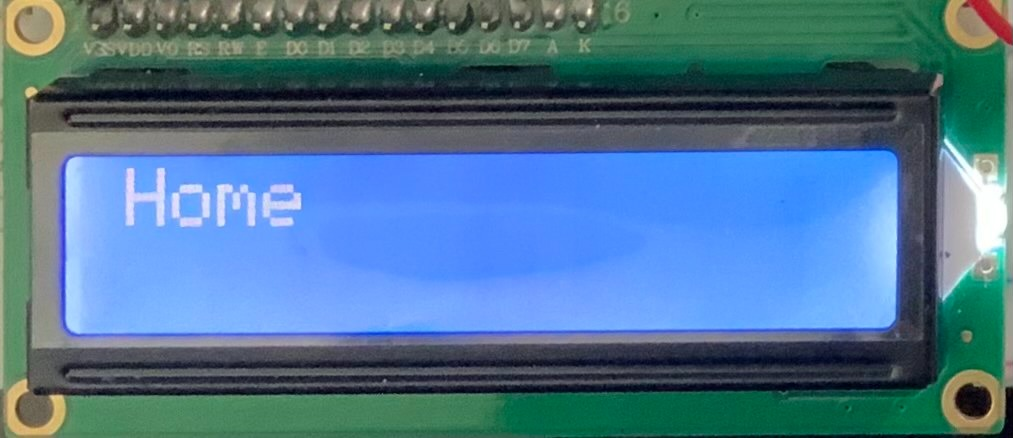
\includegraphics[width=0.7\linewidth]{Home.jpg}
  \caption{LCD Displaying only One Word}
  \label{fig:fig10}
\end{figure}

\subsection{Prevent Anymore Inputs}
If you find yourself in case similar to Figure 10, where you only want to create one word, you 
can ensure there will be no furter letters added to the screen by just pressing the "Done" button
since it takes care of both rows of the LCD screen by adding extra spaces to meet the 5 letter 
limit for each row. The extra spaces are what prevents any further inputs since you
cannot go over the 5 letter limit.


\section{Limitations}
The ASCII LCD Display is designed for those who know the American English language,
as the ASCII letters are those in the US American alpahbet. There is another 
limitation in that those with limited hand-eye coordination and/or shaky
hands can have trouble pressing the buttons and switching the switches since the buttons 
are sensitive and if pressed for too long will cause the LCD screen to display the 
same letter multiple times and the switches require one to switch the switch up and down
if needed. There is also the issue of setting up the board if one does
not understand how to load software onto the Basys 3 board or Arduino Mega and if one 
has not had practiced wiring a circuit on a breadboard before. However, other then
not having experience with the American English language, having limited motor skills, 
or not having experience with wiring a circuit then the design can work as intended.


\section{Acknowledgements}
I want to thank Ralph Heymsfeld for inspiring this project with his \href{http://robotics.hobbizine.com/fpgalcd.html}{article}.
I also want to thank Dr. Benson and the CPE Faculty for providing me with the opportunity to create this project. 
Additionally, I want to thank PIJA Education for their 
\href{https://pijaeducation.com/arduino/lcd-16x2-with-arduino-uno/print-ascii-characters-on-lcd-16x2-using-arduino/}{article}
that has provided me with the insight on how to use the LCD library on the arduino, wire the LCD to the Arduino Mega, and display letters on the screen.
I also want to thank my family for funding and testing this project. Lastly, the creation of this user manual, structual model, FSM, System Verilog code, product, 
and Arduino code is by Luis D. Garcia.
\end{document}
